% !TEX program = xelatex
% Example: PGFPlots bar chart
\documentclass[11pt, a4paper]{article}
\usepackage{pgfplots}
\pgfplotsset{compat=1.18}

\begin{document}

\section*{مخططٌ أعمدةٌ بـ PGFPlots}

% مخططُ أعمدةٍ مجمّعة
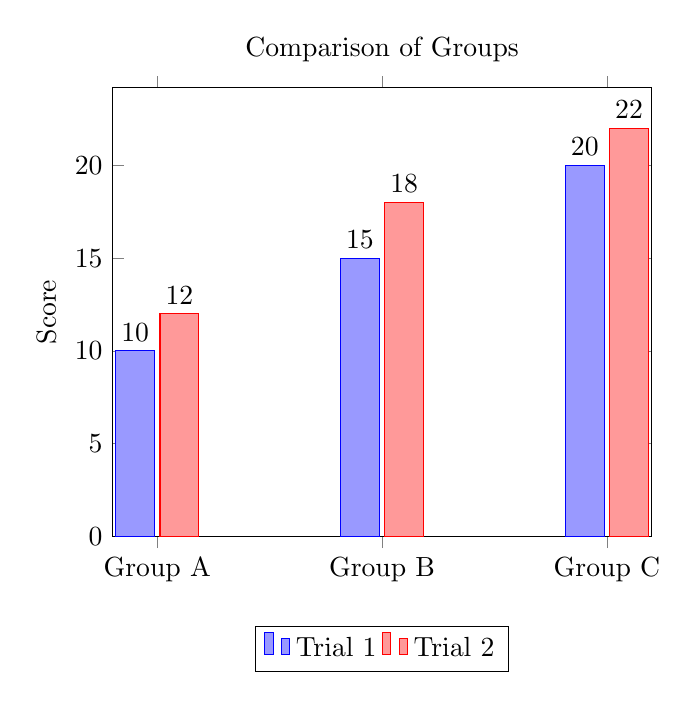
\begin{tikzpicture}
\begin{axis}[
  ybar,
  bar width=14pt,
  symbolic x coords={Group A, Group B, Group C},
  xtick=data,
  ymin=0,
  ylabel={Score},
  title={Comparison of Groups},
  legend style={at={(0.5,-0.2)}, anchor=north, legend columns=-1},
  nodes near coords,
  nodes near coords align={vertical}
]
  \addplot[fill=blue!40, draw=blue] coordinates {
    (Group A, 10) (Group B, 15) (Group C, 20)
  };
  \addlegendentry{Trial 1}

  \addplot[fill=red!40, draw=red] coordinates {
    (Group A, 12) (Group B, 18) (Group C, 22)
  };
  \addlegendentry{Trial 2}
\end{axis}
\end{tikzpicture}

\end{document}
